\chapter{Implementation}

This Chapter describes the details of the implementation, problems and limitations that may arise using the developed work.



\section{Compression}
\label{section:impl_compression}

To compress a BTF data we used Java programming language. In our case, the main problem of PCA implementation lies in employing a singular value decomposition (SVD).
To solve this problem, we used a fast linear library \emph{jblas} \cite{jblas} developed by Mikio Braun. The \emph{jblas} library is gaining popularity in scientific computing.
This library is one of the most fastest library for the Java programming that can solve various linear algebra problems. 

A compressed data has to be sent to a shader. The best way to send arrays of data to a shader, is to send them as textures. 
So, after we perform a SVD, we save our resulted matrices $U$, $\Sigma$, $V$ as textures.  Matrices $U$ and $V$ are in range $[-1;1]$, so we map the data to an image domain $[0;1]$.
We store each component of matrix $U$ separately as PNG images. We save each component separately as we would need to stream the data in pieces.

Consider the examples shown in Figure \ref{fig:compr}, which represents first components of some materials.
Matrices $\Sigma$ and $V$ are stored together in one texture as they are small enough. Note that the values of matrix $\Sigma$ are not in range $[-1;1]$, but we are still able to map them and store in the texture.
We will not go in details here, as it is a trivial task.

Also, one practical consideration when using \emph{jblas} is to scale the data for better reconstructed quality in a shader. We found out that tenths of values of $U$ and $V$ matrices are zeros.
So, basically we can scale matrices by multiplying them with $10$ and at the same time matrix $\Sigma$ by $0.1$. 
Because, the texture stores only 8-bit values, means that the data loss during mapping is inevitable for some values. 
At least, with scaling we found that we improve the precision of the decompressed data.




\begin{figure}[h]
 \centering
 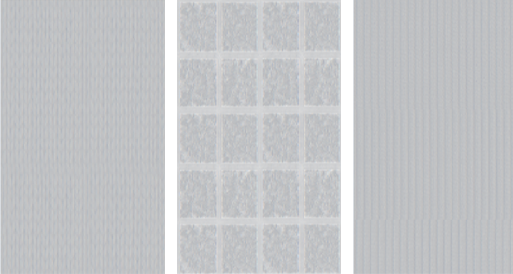
\includegraphics[width=0.7\textwidth]{figures/compr}
 \caption[Example of Principal Components] {
 	{\bf Example of Principal Components }
	
	\textbf{From left to right}: wool, impalla, corduroy. 
 }
 \label{fig:compr}
\end{figure}


\section{Rendering}
\label{section:impl_rendering}


The aim of this thesis was to implement efficient BTF-shader for XML3D \cite{xml3d}. 
XML3D platform was implemented to deploy 3D graphics in web browsers.
 This technology is based on WebGL and JavaScript. 
 BTF-shader is written in OpenGL Shading Language (GLSL). 
The rendering process of the shader is depicted in Figure \ref{fig:shader}.


A compressed BTF data is stored in two textures, which are passed to a shader. First texture $L$ stores principal components, the other $R$ stores PCA weights, which determine how the components have to be summed up.
The other inputs are texture coordinates, eye and light positions. Eye and light positions are transformed to spherical coordinates.
 Then, we lookup three closest views $A$, $B$, $C$ from the measured BTF data, which are will be needed for interpolation purpose.
 This lookup process is fairly simple. We have a static array in the shader, which stores sample intervals of the measured BTF data.
 Knowing intervals we can find the closest view positions.
 Finally, we employ barycentric coordinates interpolation for the closest eye and light positions and obtain interpolation weights $w_{o}$ and $w_{i}$ accordingly. 
 
 Meanwhile, we have to find appropriate principal components, i.e. to find the index of the texture that was sampled with given eye and light positions.
 For given eye and light positions we lookup a suitable texture index out of $3\times81\times81$ texture indices. In other words, we find which PCA weights from input texture $R$ we need. 
 Finally, texture coordinates specify which exactly pixel has to be decompressed from the texture domain, i.e. which principal components from input texture $L$ has to be used.
 Combining PCA weights with principal components we get uninterpolated color. 
 
 In a final step, uninterpolated colors are then combined with earlier found interpolation weights to get the final color.
 
 
The implemented shader has the it's own limitations. 
First of all, the number of principal components has to be fixed for a shader, because WebGL does not allow dynamic loops.
Secondly, number of principal components are bound by a size of a texture $L$. It means not all GPUs can handle very big textures, so it must be considered beforehand.
For example, the texture of size 4096MB can store 8 components with subset size of 3. Such size can handle average GPU.
Last but not least, the array of sample intervals of the BTF are pre-compiled with a shader.
For the BTF Bonn database all materials were sampled under the same intervals.

 


\begin{figure}[h]
 \centering
 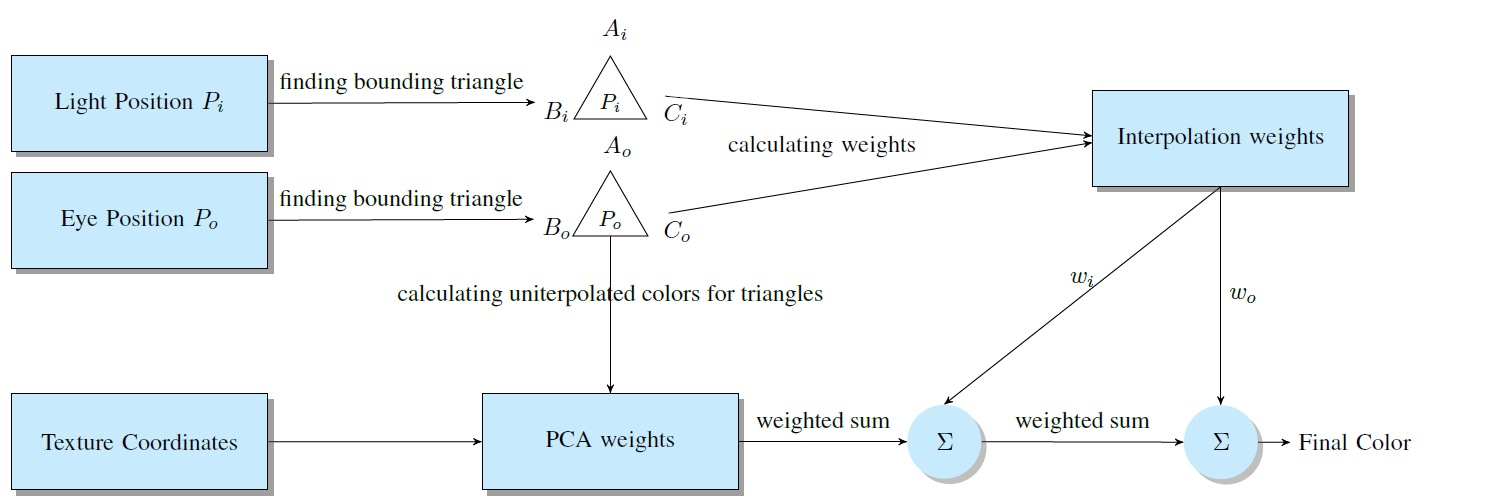
\includegraphics[width=1.0\textwidth]{figures/shader}
 \caption[Shader Design] {
 	{\bf Shader Design }

 }
 \label{fig:shader}
\end{figure}


\section{Streaming}
\label{section:impl_streaming}

As for streaming solution we used Node.js\cite{nodejs} platform, which is written in JavaScript.
 Node.js allows to write efficient web applications that is event-driven and employs a non-blocking I/O model.
On top of that, we employ BinaryJS\cite{binaryjs} library for Node.js, which provides us with binary streaming using web-sockets.


Node.js server is independent from main web server where an user browsers 3D content.
After the user connects and the page completely loads, JavaScript client side requests Node.js server to start streaming BTF data.
That means that all compressed BTF data are located on the Node.js server.

We also use Xflow\cite{xflow} tool for a client side.
Xflow is a part of XML3D implementation, which allows to process data on flow, i.e. in runtime.
So, we use Xflow for saving all newly arrived principal components in texture $L$ on a client side. Figure \ref{fig:streaming} depicts the streaming process.

\begin{figure}[h]
 \centering
 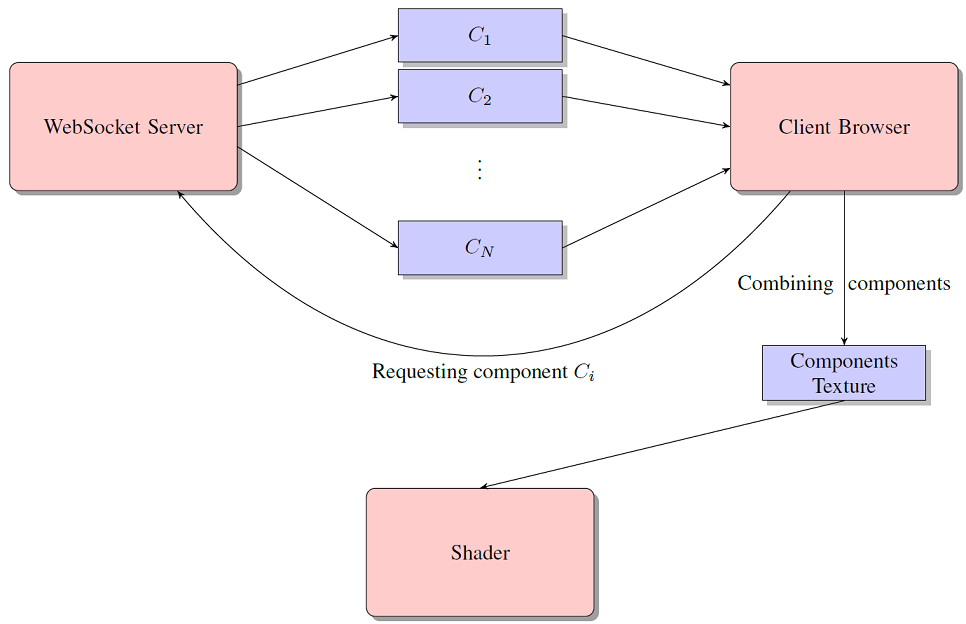
\includegraphics[width=1.0\textwidth]{figures/streaming}
 \caption[Streaming process illustration ] {
 	{\bf Streaming process illustration}
	}
 \label{fig:streaming}
\end{figure}


At the start of a stream, we first send texture $R$ and meta data to the client side. 
Then, on the client side we create array with the name \emph{texData}. This array stores RGB colors, which further will be passed as texture $L$ to the shader.
As it was described in chapter \ref{section:streaming}, we stream principal components $C_{i}$ one by one.
Each principal component $C_{i}$ for all possible sampled views are streamed as PNG image. 
Node.js server streams images in chunks, which permits client side other processing to continue before the whole transmission of PNG image is finished.

Then, on a client side we decode PNG image using PNG decoder written in JavaScript by Arian Stolwijk \cite{pngreader}.
PNG images are decoded to pure array of RGB colors and stored in its place in \emph{texData} array. 
Finally, using Xflow from \emph{texData} array we create texture $L$, with which we update our BTF-shader.



\label{chapter:implementation}
